\documentclass[conference,a4paper]{IEEEtran}
\IEEEoverridecommandlockouts
\usepackage{cite}
\usepackage{graphicx,amsmath,amssymb,booktabs,array,url,balance}
\usepackage{xurl}
\setlength{\textfloatsep}{7pt plus 2pt minus 2pt}
\setlength{\floatsep}{6pt plus 2pt minus 2pt}
\setlength{\intextsep}{5pt plus 2pt minus 2pt}
\renewcommand{\arraystretch}{1.06}
\begin{document}
\title{When Does Waiting Help? Observable-History Retry Control for API-Dependent Agentic AI Workflows}
\author{\IEEEauthorblockN{Yukai Zeng}\IEEEauthorblockA{Singapore Ministry of Defence Communications Organisation (MCO)}}
\maketitle
\begin{abstract}
Agentic AI workflows depend on networked search, retrieval and checking services. When a call fails, the client cannot tell an independent fault from a shared outage. A simulator can, and letting a policy see that distinction distorts how it is judged. In our seeded workflow simulator, a policy that reads the hidden outage label delivered 92.0\% of briefs on time and fresh, but only 24.5\% once outages were masked as ordinary 5xx responses. We therefore test a three-parameter controller that chooses between a short and a long wait using only status codes, \texttt{Retry-After} hints and its last 6~s of responses. Tuned on development data and then frozen, it was compared with four baselines in 15,000 held-out trials on three strategic-communications reporting workflows, 3,600 trials on unseen graphs and 320 localhost HTTP runs. The controller stayed within 1.5 percentage points of exponential backoff in every held-out condition and beat it by 21--38 points under a masked extended outage. On average it did no better than a conservative linear cooldown, which recovered more of outages 1--3~s longer than in development, while the controller did better under independent faults. Immediate retry beat both whenever faults were independent. Scored against the hidden label, the controller chose its long wait for 64\% of outage-driven retries and for up to 26\% of retries after independent errors. With perfect detection, the same two waits would draw level with the cooldown in two of three workflows but still trail immediate retry under tight deadlines.
\end{abstract}

\begin{IEEEkeywords}
agentic AI workflows, retry control, fault tolerance, HTTP 429 and 503, circuit breaker, quality of service
\end{IEEEkeywords}

\section{Introduction}
An AI agent that searches for, retrieves and cross-checks sources makes many calls to networked tools, and some of those calls fail. Retrying improves the chance of finishing, but each retry spends time and request capacity. In time-sensitive work such as information-environment assessment, an AI support capability identified by the NATO StratCom Centre of Excellence \cite{nato}, a slow retrieval can also leave material out of date by the time a brief reaches the analyst who reviews it. We study the reliability of the computing pipeline behind such assessments.

Agent benchmarks such as AgentBench and $\tau$-bench measure how well agents complete multi-step tasks with tools \cite{agentbench,taubench}. Newer benchmarks inject tool faults such as timeouts and rate limits, and find that agent performance drops under them \cite{reliabilitybench,toolbenchx}. Those studies evaluate the agent itself. We look at a narrower layer: how an agent's tool client should respond when a call fails. Adapting retries to observed history is an old idea in networking. TCP sets its retransmission timeout from smoothed round-trip measurements and doubles it after each expiry \cite{rfc6298}. Systems research has also shown that retries add tail latency and load \cite{tail,brooker} and can keep an overloaded service from recovering \cite{bronson,huang}. In response, production clients cap retries with budgets \cite{sre}, throttle them when failures accumulate \cite{grpc,awsretry}, or stop calling a failing service with a circuit breaker \cite{nygard,resilience4j}. All of these mechanisms act only on what the client can observe.

\begin{table}[t]
\centering
\caption{Label-masking control: timely fresh delivery (\%, 200 seeds) when the outage cause is visible to the policy (Vis.) or reported as a generic 5xx (Mask.). 45-s deadline, 8\% background errors, unextended outages.}
\label{tab:mask}
\scriptsize
\setlength{\tabcolsep}{3.5pt}
\begin{tabular}{@{}lrrcrrcrr@{}}\toprule
 & \multicolumn{2}{c}{IEA} && \multicolumn{2}{c}{LFC} && \multicolumn{2}{c}{CSR}\\
\cmidrule(lr){2-3}\cmidrule(lr){5-6}\cmidrule(lr){8-9}
Policy & Vis. & Mask. && Vis. & Mask. && Vis. & Mask.\\\midrule
Immediate & 25.5 & 25.5 && 13.0 & 13.0 && 27.0 & 27.0\\
Exponential backoff & 70.5 & 70.5 && 68.0 & 68.0 && 72.0 & 72.0\\
Cause-aware & 92.0 & 24.5 && 83.0 & 12.5 && 92.0 & 26.5\\
Linear cooldown & 93.5 & 93.5 && 72.0 & 72.0 && 91.5 & 91.5\\\bottomrule
\end{tabular}
\end{table}


A retry policy can look strong in simulation simply because it reads the simulator's outage label, which a real client never receives. Table~\ref{tab:mask} shows the size of the effect (Section~\ref{sec:sim}; seeds 2026--2225, 200 per cell). The cause-aware policy in the table waits $1.5a$~s after a failure labelled \texttt{outage} and $0.2a$~s after any other 5xx or timeout, where $a$ is the attempt number; it also caps calls per workflow and skips retries that a critical-path estimate says cannot finish in time. With the label visible, it delivered 92.0\% of information-environment briefs on time and fresh. When the same outages were reported as ordinary 5xx responses, it delivered 24.5\%, and the other two workflows fell by similar margins. Immediate retry, exponential backoff and linear cooldown never read the label, and their outcomes were identical seed for seed in both conditions. The cause-aware policy's result therefore depended entirely on the label. The label-blind linear cooldown, which waits long after every 5xx, matched it in IEA and CSR, but Section~\ref{sec:heldout} shows that it pays for this under independent faults. The rest of the paper asks whether a client that sees only its own recent responses can wait long only when it should.

The paper makes three contributions. First, the label-masking control shows how easily a retry evaluation can hand a policy information that a real client lacks. Second, we tune a three-parameter controller on development data, freeze it, and compare it with four baselines on held-out workflows, unseen graph shapes and real localhost HTTP requests. No policy, the controller included, wins every condition. Third, four post-hoc diagnostics explain where it falls short: sweeps over outage length and history window, a check of the controller's outage detection, and an ablation that compares the controller with its two waits used alone and with perfect detection. The workflows are simulated; the HTTP runs target a local server, and no experiment involves language-model inference, fact verification or production traffic.

\section{Retry Policies Compared}
HTTP 429 tells a client that it is being throttled, and a \texttt{Retry-After} header can say how long to wait \cite{rfc6585,rfc9110}. AWS SDKs pair jittered exponential backoff with a retry quota and an optional adaptive rate limiter \cite{awsretry}. gRPC suspends retries to a server once too many recent calls to it have failed \cite{grpc}, and circuit breakers open when the failure rate over a sliding window passes a threshold \cite{resilience4j}. Our controller belongs to this family and uses no new detection mechanism; the contribution is a controlled comparison in which every policy sees the same information and is scored on whether a dependent workflow delivers fresh results on time.

\begin{table}[t]
\centering
\caption{Retry delay schedules. $a$: attempt number; $j\in[0.85,1.15]$: seeded jitter; $n$: task count. Sums are over three retries, before jitter.}
\label{tab:delays}
\scriptsize
\begin{tabular}{@{}lll@{}}\toprule
Policy & Delay before next attempt (s) & $\Sigma$ (s)\\\midrule
Immediate & 0 (ignores \texttt{Retry-After}) & 0\\
Exponential backoff & $\min(8,\,0.8\cdot2^{a-1})\,j$ & 5.6\\
SDK-style proxy & exponential, plus call cap $\lfloor1.8n+0.5\rfloor$ & 5.6\\
Linear cooldown & $\min(5,\,1.5a)\,j$; timeouts $0.2a\,j$ & 9.0\\
History-adaptive & $\min(5,\,\beta a j)$, $\beta\in\{0.4,2.0\}$ by Eq.~(\ref{eq:delay}) & 2.4 / 11.0\\\bottomrule
\end{tabular}
\end{table}

Table~\ref{tab:delays} lists the five policies. After a 429, every policy except Immediate waits at least as long as \texttt{Retry-After} asks. Permanent errors are never retried, and no task gets more than four attempts. With that limit, the longest total wait in the table (11~s) still fits inside the shortest held-out deadline (14~s). The SDK-style proxy is exponential backoff plus a cap on calls per workflow; it does not run an AWS SDK or reproduce its token accounting. All policies see timestamps, task dependencies, status codes and \texttt{Retry-After} values. None sees the true service state or any future draw.

\section{Workflow Simulator and Controller}\label{sec:sim}
\subsection{Synthetic reporting workflows and metric}
We use three fixed directed acyclic graph (DAG) templates: information-environment assessment (IEA, 10 tasks), live fact-check support (LFC, 8) and communications situation reporting (CSR, 9). Each follows the generic stages of an assessment brief (Fig.~\ref{fig:workflow}): public-source retrieval, mandatory provenance and consistency checks, optional enrichment, and handoff to a human-review queue. The templates do not reproduce any organisation's procedure.

\begin{figure}[t]
\centering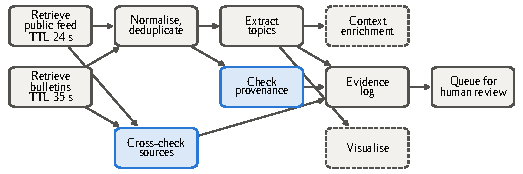
\includegraphics[width=\columnwidth]{figures/workflow_structure.pdf}
\caption{IEA template (ten tasks). Dashed: optional; shaded: checks; TTL: freshness limit. A completed check means only that the task ran.}
\label{fig:workflow}
\end{figure}

Let $D_s^\pi$ indicate brief delivery for seed $s$ and policy $\pi$, $M_s^\pi$ completion of the required checks, $\Delta$ the deadline, and $R$ the set of mandatory retrievals, each with a freshness TTL $\tau_i$ (20--35 simulated seconds, chosen for illustration and not calibrated). With $t_s^\pi$ the delivery time and $t_{i,s}^\pi$ the completion time of retrieval $i$, the endpoint is timely fresh delivery
\begin{equation}\label{eq:metric}
Y_s^\pi=\mathbf{1}\!\left[D_s^\pi\land M_s^\pi\land t_s^\pi\le\Delta\land\bigwedge_{i\in R}(t_s^\pi-t_{i,s}^\pi\le\tau_i)\right].
\end{equation}
For policies $A,B$, the paired effect is $\widehat\delta_{A,B}=N^{-1}\sum_s(Y_s^A-Y_s^B)$, with 95\% percentile bootstrap intervals that resample seeds \cite{efron}.

For each seed, every task has fixed error and latency draws for each attempt, with latencies from a bounded log-normal distribution (median 1.25~s). Four workers execute the DAG as a discrete-event simulation. Each seed also has two shared outage windows: one of 6.5~s starting between 4.5 and 7.5~s, and one of 3.0~s starting between 19 and 23~s. Any request sent during a window fails fast (0.2~s) with a 5xx. All policies share the same draws, but outages and the 429 token bucket depend on when a request is sent, so two policies can meet different failures on the same seed.

\subsection{Observable-history retry controller}
At time $t$, let $H_t$ hold the \emph{completed} responses $(u,z)$ from the preceding $W=6$~s of the same workflow, where $u$ is the completion time and $z$ the outcome. We set $W$ before tuning to just under the 6.5-s first outage window, a choice informed by the simulator; Section~\ref{sec:window} tests 2 and 12~s. Let $e_t=\sum_{(u,z)\in H_t}\mathbf{1}[z\in\{\mathrm{5xx},\mathrm{timeout}\}]$ count the recent 5xx responses and timeouts. After a retryable 5xx or timeout at attempt $a$, the controller waits
\begin{equation}\label{eq:delay}
d(t,a)=\min\!\left(5, a\,j\left[\,\beta_{\rm long}\,\mathbf{1}(e_t\ge k)+\beta_{\rm short}\,\mathbf{1}(e_t<k)\right]\right)\ \text{s}.
\end{equation}
After a 429 it waits $\max(0.8a,r)$~s, where $r$ is the \texttt{Retry-After} value. It also skips any retry that would leave less than 0.1~s before the deadline; this guard changed no outcome in the 3,000 held-out history-adaptive trials.

\section{Evaluation Protocol}
\subsection{Development tuning, then freeze}
A development grid crossed $k\in\{2,3\}$, $\beta_{\rm short}\in\{0.2,0.4\}$ and $\beta_{\rm long}\in\{1,1.5,2\}$ with $W=6$~s fixed: 12 configurations $\times$ 360 trials (three templates, three development conditions, 40 seeds) $=4{,}320$ records. The development conditions were 22\% IID errors with a 22-s deadline, an unextended outage with 7\% background errors, and a hinted 1.8 requests/s quota. Selection used pooled timely fresh delivery, with mean calls as a tie-break, and chose $k=3$, $\beta_{\rm short}=0.4$, $\beta_{\rm long}=2.0$ (96.1\% on development data). We froze that setting in a JSON file before running any held-out trial. A post-hoc 120-configuration grid on the same development seeds ($k\le5$, $\beta_{\rm short}\le1.5$, $\beta_{\rm long}\le3$) still ranked it first, so a wider search over these ranges would not have changed the choice.

\subsection{Held-out and structural tests}
Five policies were run on three templates and five held-out conditions, each with 200 new seeds ($5\times3\times5\times200=15{,}000$ records): independent and identically distributed (IID) errors at 27\%, a masked outage with both windows extended by 2~s, tight IID errors (17\%, 14-s deadline), a hinted quota (2.3 requests/s) and mixed permanent/transient errors. The tight-deadline and mixed conditions have no counterpart in development. A further 3,600 records (three topologies $\times$ two failure conditions $\times$ five policies $\times$ 120 seeds) use unseen 8-node chains, 15-node fan-outs and 18-node layered DAGs. These graphs are scored by \emph{generic completion} rather than freshness. Seed ranges for development, held-out, structural and HTTP runs do not overlap.

\subsection{Localhost HTTP integration test}
A standard-library server and client exchanged real requests over \texttt{127.0.0.1}, with injected 503s, 429s carrying \texttt{Retry-After}, timeouts and a brief outage. Each of the 320 records (four regimes $\times$ five policies $\times$ 16 seeds) is a workflow of three sequential calls, with time accelerated to 35~ms per nominal second.

\subsection{Post-hoc diagnostics}
Four further analyses used the held-out seeds after the primary test, and none fed back into the configuration: an outage-length sweep (extensions of 0--6~s, 18,000 records, whose +2-s slice matches the primary records exactly); a history-window sweep ($W\in\{2,6,12\}$~s, 3,600 records); a detector check that uses the hidden outage label \emph{only to score} the controller's state; and a switching ablation (18,000 records) that runs the controller with its short or long wait alone and with perfect outage detection, which reads the hidden label and serves only as an upper bound.

\section{Results}
\subsection{Held-out rankings}\label{sec:heldout}
\begin{table*}[t]
\centering
\caption{Held-out timely fresh delivery (\%, $N=200$ matched seeds per cell). Deadlines and background errors: IID, 26~s; extended outage, 48~s, 10\% IID; tight, 14~s; hinted quota (2.3 requests/s), 52~s, 9\% IID; mixed, 40~s, 20\% IID and 2\% permanent. Imm.: immediate; Exp.: exponential backoff; SDK: SDK-style proxy; Cool.: linear cooldown; Hist.: history-adaptive. Bold: best in the row within each workflow, ties included.}
\label{tab:main}
\footnotesize
\setlength{\tabcolsep}{3.4pt}
\begin{tabular}{@{}l*{5}{r}c*{5}{r}c*{5}{r}@{}}\toprule
 & \multicolumn{5}{c}{IEA} && \multicolumn{5}{c}{LFC} && \multicolumn{5}{c}{CSR}\\
\cmidrule(lr){2-6}\cmidrule(lr){8-12}\cmidrule(lr){14-18}
Condition & Imm. & Exp. & SDK & Cool. & Hist. && Imm. & Exp. & SDK & Cool. & Hist. && Imm. & Exp. & SDK & Cool. & Hist.\\\midrule
IID 27\% & \textbf{95.0} & 92.5 & 92.5 & 87.0 & 93.0 && \textbf{95.5} & 89.0 & 89.0 & 81.0 & 87.5 && \textbf{94.0} & 92.0 & 91.0 & 87.5 & 91.5\\
Extended outage & 26.0 & 23.0 & 23.0 & \textbf{74.0} & 60.5 && 16.0 & 18.5 & 18.5 & \textbf{66.0} & 39.5 && 25.5 & 23.0 & 23.0 & \textbf{75.0} & 51.5\\
Tight IID 17\% & \textbf{95.0} & 78.5 & 78.5 & 71.5 & 80.5 && \textbf{91.0} & 76.0 & 76.0 & 65.0 & 81.0 && \textbf{93.5} & 75.5 & 75.5 & 69.0 & 78.5\\
Hinted quota & 41.5 & \textbf{99.5} & \textbf{99.5} & 98.0 & 99.0 && \textbf{99.5} & \textbf{99.5} & \textbf{99.5} & 98.5 & \textbf{99.5} && 0.0 & \textbf{100.0} & \textbf{100.0} & 99.0 & \textbf{100.0}\\
Mixed permanent & \textbf{83.5} & 82.5 & 82.5 & 81.0 & 82.5 && \textbf{84.5} & 82.0 & 81.5 & 79.5 & 82.0 && \textbf{82.0} & 81.5 & 81.0 & 80.0 & 81.5\\\bottomrule
\end{tabular}
\end{table*}


Table~\ref{tab:main} gives all fifteen held-out cells, and Fig.~\ref{fig:paired} gives the paired intervals for the two conditions that separate the policies most. History-adaptive retry was never more than 1.5 points behind exponential backoff (LFC, 27\% IID), the usual SDK default \cite{awsretry,grpc}, and was far ahead of it under the extended outage, by 21.0 to 37.5 points across the three workflows. Under tight deadlines it was 2 to 5 points ahead of backoff, though the interval excludes zero only in LFC. The linear cooldown recovered more of the extended outage in every workflow (74.0\% against 60.5\% in IEA), and immediate retry delivered more in every independent-fault condition, most of all under tight deadlines (95.0\% against 80.5\% in IEA). No policy was best in every condition: history-adaptive retry never won a condition outright, but no other policy beat it in all five. Averaged over the fifteen cells, it fell 8.0 points short of each cell's best policy, against 7.7 for the linear cooldown, 14.3 for exponential backoff and 20.4 for immediate retry. Because immediate retry ignores \texttt{Retry-After}, its results under the hinted quota swing with the workflow, from 99.5\% in LFC to 0.0\% in CSR. The SDK-style proxy's call cap bound in only 12 of the 3,000 held-out trials and changed the outcome in four, so the proxy otherwise matched exponential backoff.

\begin{figure}[t]
\centering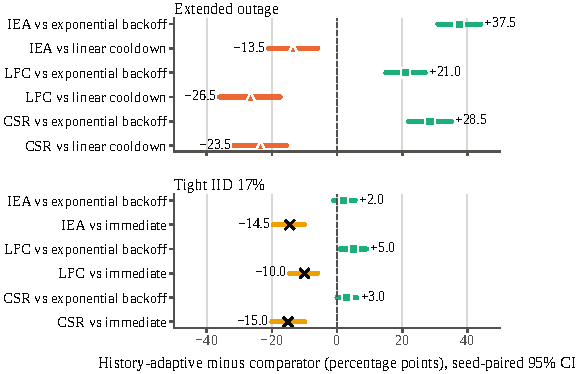
\includegraphics[width=\columnwidth]{figures/heldout_differences.pdf}
\caption{Seed-paired 95\% intervals for history-adaptive minus each comparator under the held-out extended outage (top) and tight deadlines (bottom).}
\label{fig:paired}
\end{figure}

\subsection{Delay budgets and outage detection}
With at most four attempts per task, a policy gets through an outage only if its waits add up to more than the outage time remaining when its first failure arrives. The held-out windows last 8.5~s and 5.0~s. Exponential backoff waits 5.6~s in total (Table~\ref{tab:delays}), which is usually too little for the longer window, while the cooldown's 9.0~s usually covers it. History-adaptive retry waits either 2.4~s or 11.0~s, so its result hinges on noticing the outage. Scored against the hidden label, it chose the long wait for 64\% of the 1,808 retries that followed outage-caused failures. It also chose the long wait after independent errors, for 26\% of those retries at the 27\% error rate and 14\% at the 17\% rate.

\begin{table}[t]
\centering
\caption{Switching ablation: timely fresh delivery (\%, 200 held-out seeds). Short and Long fix the controller's wait at $0.4a$ or $2.0a$~s; Perfect picks between them using the hidden outage label, as an upper bound. Cool.\ and Imm.\ as in Table~\ref{tab:main}. Bold: best in the row.}
\label{tab:switch}
\scriptsize
\setlength{\tabcolsep}{3.2pt}
\begin{tabular}{@{}llrrrrrr@{}}\toprule
Condition & & Hist. & Short & Long & Perfect & Cool. & Imm.\\\midrule
Extended outage & IEA & 60.5 & 23.5 & 70.0 & \textbf{75.0} & 74.0 & 26.0\\
 & LFC & 39.5 & 14.5 & 48.5 & 57.5 & \textbf{66.0} & 16.0\\
 & CSR & 51.5 & 22.5 & 64.0 & \textbf{76.0} & 75.0 & 25.5\\
\addlinespace
Tight IID 17\% & IEA & 80.5 & 87.0 & 60.0 & 87.0 & 71.5 & \textbf{95.0}\\
 & LFC & 81.0 & 84.0 & 58.0 & 84.0 & 65.0 & \textbf{91.0}\\
 & CSR & 78.5 & 84.5 & 62.5 & 84.5 & 69.0 & \textbf{93.5}\\\bottomrule
\end{tabular}
\end{table}


Table~\ref{tab:switch} separates the cost of these errors from the cost of the waits themselves. Used alone, the short wait collapses under the extended outage (14.5--23.5\%), and the long wait loses 16 to 23 points to the controller under tight deadlines. In every held-out cell, the controller's result lies between the two. With perfect detection, the same waits would draw level with the cooldown under the extended outage in IEA and CSR (paired differences of +1.0 points, with intervals spanning zero) and recover about two-thirds of the gap in LFC, so detection errors explain most of the outage loss in Section~\ref{sec:heldout}. Under tight deadlines, perfect detection only reaches the short wait's result, which is still 7 to 9 points behind immediate retry. False alarms therefore explain less than half of that gap; the rest is the cost of waiting at all.

\begin{figure*}[t]
\centering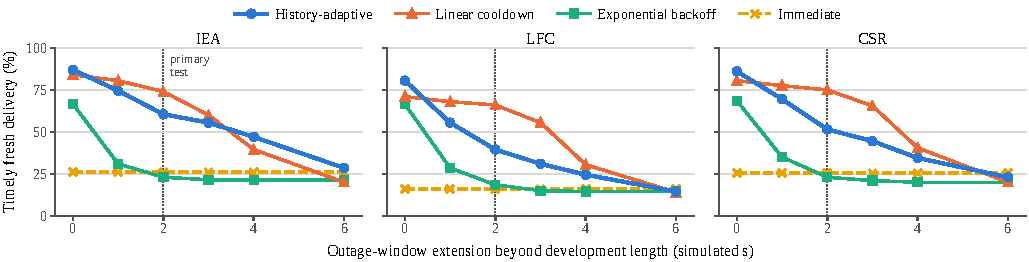
\includegraphics[width=\textwidth]{figures/outage_duration.pdf}
\caption{Post-hoc outage-length sweep (200 held-out seeds per point). The +2-s point is the primary test. The SDK-style proxy overlaps exponential backoff and is omitted.}
\label{fig:outage}
\end{figure*}

\subsection{Outage-length sensitivity}
Fig.~\ref{fig:outage} repeats the outage test with both windows lengthened by 0, 1, 2, 3, 4 or 6~s. The primary +2-s condition turns out to be where the cooldown's lead is largest. At the development length (+0~s), history-adaptive retry was ahead of the cooldown in all three workflows, by 3.0 to 9.5 points, with intervals excluding zero in LFC and CSR. With 1--3~s of extension the cooldown led; its interval excluded zero at every one of those lengths in LFC and CSR, but in IEA only at +2~s. At +4 and +6~s history-adaptive retry moved ahead again in IEA, while the other two workflows were too close to separate. By +6~s the first outage outlasted every policy's total wait, and in LFC and CSR immediate retry did as well as any waiting policy. Exponential backoff fell from 66.5\% to 31.0\% in IEA with a single extra second of outage, and history-adaptive retry stayed at or above it at every length. Whether the cooldown or the controller comes out ahead depends on how long an outage lasts compared with each policy's total wait.

\subsection{Unseen graph topologies}
On the unseen chain, fan-out and layered graphs (120 seeds each), history-adaptive retry completed 76--91\% of workflows under outages, against 35--68\% for exponential backoff (paired gains of 23 to 41 points) and 0--47\% for immediate retry. It matched the linear cooldown to within one point on every graph. Under independent errors the policies were indistinguishable, except that the proxy's call cap cost it two chain workflows.

\subsection{History-window sensitivity}\label{sec:window}
A longer history window helps under outages and hurts under independent errors. In IEA, moving from $W=2$ to 12~s lowered delivery under independent errors from 95.0\% to 87.0\% and raised it under the extended outage from 40.0\% to 63.0\%; LFC and CSR moved the same way. A longer memory treats scattered independent errors as a sign of an outage. Both $W$ and $k$ would need calibrating against real traffic before deployment.

\subsection{Localhost HTTP integration test}
\begin{table}[t]
\centering
\caption{Localhost HTTP: workflow completion, \% (mean requests). 16 runs per cell; injected faults, not provider traces. Abbreviations as in Table~\ref{tab:main}. $^{*}$Seed-independent schedule: one deterministic scenario repeated 16 times.}
\label{tab:http}
\scriptsize
\setlength{\tabcolsep}{3pt}
\begin{tabular}{@{}lrrrrr@{}}\toprule
Regime & Imm. & Exp. & SDK & Cool. & Hist.\\\midrule
IID 503 & 93.8 (4.0) & 93.8 (4.0) & 87.5 (3.9) & 93.8 (4.0) & 93.8 (4.0)\\
Brief 503 outage$^{*}$ & 0.0 (4.0) & 100 (6.0) & 100 (6.0) & 100 (5.0) & 100 (6.0)\\
Shared 429$^{*}$ & 0.0 (5.0) & 100 (5.0) & 100 (5.0) & 100 (5.0) & 100 (5.0)\\
Injected timeout & 100 (3.8) & 100 (3.8) & 93.8 (3.7) & 100 (3.8) & 100 (3.8)\\\bottomrule
\end{tabular}
\end{table}

Table~\ref{tab:http} shows that the decision code used in simulation also handles real status codes, \texttt{Retry-After} headers and client timeouts. Every waiting policy got through the brief outage and the shared 429 limit and immediate retry did not, so the test cannot rank the waiting policies. In the IID and timeout regimes, the proxy's call cap stopped one more workflow than the other policies.

\section{Limitations and Reproducibility}
The DAGs, TTLs, deadlines and outage windows are illustrative rather than calibrated. The intervals describe seed-to-seed variation within our generator, and the exploratory comparisons are not corrected for multiplicity. The most important missing element is load feedback. Outages are scheduled in advance, so retries can never prolong them, and the retry storms and metastable overload described in \cite{bronson,huang} cannot arise. A service that slows down under retry traffic could reorder the policies. The controller's history is also reset for each workflow, whereas a client-wide history shared across concurrent workflows, of the kind a circuit breaker keeps, might detect outages sooner.

All simulated tasks are idempotent. Real tools may publish, submit or update records, and a deployed retry layer would need idempotency keys or operator review before repeating such calls. Freshness is measured by time alone, so $Y=1$ means a brief arrived on time from recent sources and says nothing about whether its content was right or approved.

The code is available at \url{https://github.com/yukai83/RetryBench-StratCom}. It contains the simulator, the frozen configuration, per-seed CSVs, audit scripts, a checker for every number quoted here, and 87 automated tests.

\section{Conclusion}
Letting a retry policy read the simulator's outage label made its outage performance look almost four times better than it was (92.0\% against 24.5\% in IEA). Without that label, a three-parameter controller driven by recent response history stayed within 1.5 points of exponential backoff in every held-out condition and beat it by 21--38 points under the masked extended outage, with similar gains on unseen graphs. On average it did no better than the linear cooldown, which did better on outages \mbox{1--3}~s longer than in development, while the controller did better under independent faults, where immediate retry beat both. Under outages the controller is limited by detection: it chose the long wait for 64\% of outage-driven retries, and perfect detection with the same waits would draw level with the cooldown in two of the three workflows. Under tight deadlines, false alarms explain less than half of its gap to immediate retry, and the rest is the cost of the short wait itself. Better detection and a shorter wait after independent errors would address these; tests against load-dependent services, real SDK and circuit-breaker implementations and permissioned response traces come next.

\section*{AI-Use Disclosure}
Claude (Anthropic) and ChatGPT (OpenAI) were used for language editing. The author reviewed all changes and takes responsibility for the content.

\balance
\begin{thebibliography}{00}
\bibitem{nato} G. Bergmanis-Kor\=ats, G. Bertolin, A. Pu\v{z}ule, and Y. Zeng, \emph{AI in Support of StratCom Capabilities}, M. Read, Ed. Riga, Latvia: NATO Strategic Communications Centre of Excellence, 2024, ISBN: \mbox{978-9934-619-55-7}.
\bibitem{agentbench} X. Liu \emph{et al.}, ``AgentBench: Evaluating LLMs as agents,'' in \emph{Proc. Int. Conf. Learn. Representations (ICLR)}, 2024.
\bibitem{taubench} S. Yao, N. Shinn, P. Razavi, and K. Narasimhan, ``$\tau$-bench: A benchmark for tool-agent-user interaction in real-world domains,'' in \emph{Proc. Int. Conf. Learn. Representations (ICLR)}, 2025.
\bibitem{reliabilitybench} A. Gupta, ``ReliabilityBench: Evaluating LLM agent reliability under production-like stress conditions,'' arXiv:2601.06112, 2026.
\bibitem{toolbenchx} Y. Tian, Z. Shi, Y. Zhou, and B. Zhao, ``Beyond function calling: Benchmarking tool-using agents under tool-environment unreliability,'' arXiv:2606.25819, 2026.
\bibitem{rfc6298} V. Paxson, M. Allman, J. Chu, and M. Sargent, ``Computing TCP's retransmission timer,'' RFC 6298, 2011, doi: 10.17487/RFC6298.
\bibitem{tail} J. Dean and L. A. Barroso, ``The tail at scale,'' \emph{Commun. ACM}, vol. 56, no. 2, pp. 74--80, 2013, doi: 10.1145/2408776.2408794.
\bibitem{brooker} M. Brooker, ``Timeouts, retries, and backoff with jitter,'' \emph{The Amazon Builders' Library}, Amazon Web Services, Dec. 2019. [Online]. Available: \url{https://builder.aws.com/content/3EumjoZascWd1oZiEgL8ORlv3qE/timeouts-retries-and-backoff-with-jitter}. Accessed: Oct. 23, 2026.
\bibitem{bronson} N. Bronson, A. Aghayev, A. Charapko, and T. Zhu, ``Metastable failures in distributed systems,'' in \emph{Proc. Workshop Hot Topics Oper. Syst. (HotOS)}, 2021, pp. 221--227, doi: 10.1145/3458336.3465286.
\bibitem{huang} L. Huang \emph{et al.}, ``Metastable failures in the wild,'' in \emph{Proc. 16th USENIX Symp. Oper. Syst. Des. Implement. (OSDI)}, 2022, pp. 73--90.
\bibitem{sre} B. Beyer, C. Jones, J. Petoff, and N. R. Murphy, Eds., \emph{Site Reliability Engineering: How Google Runs Production Systems}. Sebastopol, CA, USA: O'Reilly Media, 2016, ch. 21.
\bibitem{grpc} N. Eisen and E. Gribkoff, ``gRPC retry design,'' gRPC proposal A6. [Online]. Available: \url{https://github.com/grpc/proposal/blob/master/A6-client-retries.md}. Accessed: Oct. 23, 2026.
\bibitem{awsretry} Amazon Web Services, ``Retry behavior,'' \emph{AWS SDKs and Tools Reference Guide}. [Online]. Available: \url{https://docs.aws.amazon.com/sdkref/latest/guide/feature-retry-behavior.html}. Accessed: Oct. 23, 2026.
\bibitem{nygard} M. T. Nygard, \emph{Release It! Design and Deploy Production-Ready Software}, 2nd ed. Raleigh, NC, USA: Pragmatic Bookshelf, 2018.
\bibitem{resilience4j} Resilience4j, ``CircuitBreaker,'' \emph{Resilience4j Documentation}. [Online]. Available: \url{https://resilience4j.readme.io/docs/circuitbreaker}. Accessed: Oct. 23, 2026.
\bibitem{rfc6585} M. Nottingham and R. Fielding, ``Additional HTTP status codes,'' RFC 6585, 2012, doi: 10.17487/RFC6585.
\bibitem{rfc9110} R. Fielding, M. Nottingham, and J. Reschke, ``HTTP semantics,'' RFC 9110, 2022, doi: 10.17487/RFC9110.
\bibitem{efron} B. Efron, ``Bootstrap methods: Another look at the jackknife,'' \emph{Ann. Statist.}, vol. 7, no. 1, pp. 1--26, 1979, doi: 10.1214/aos/1176344552.
\end{thebibliography}
\end{document}
